\newpage
\section{Simulation Analysis}
\label{sec:simulation}


\subsection{Audio Amplifier Circuit}

The objective of this laboratory assignment is to design an Audio Amplifier circuit, using the a Gain Stage and Output Stage. The Gain Stage objective is to increase the gain, and the output stage purpose is to decrease the output impedance.




\subsection{Input Signal}

The entry signal was computed as a sinusoidal Voltage Source with an amplitude of 10 mV. Besides that, a resistor was implemented to make the simulation behaviour more similar to the real one.



\subsection{Gain Stage}

The objective of the Gain  Stage, as is stated in the name, is to amplify the input signal. With this objective in view, the circuit shown below was implemented: 


\begin{figure}[H] \centering
\includegraphics[width=1.1\linewidth]{Gain.pdf}
\caption{Implemented Gain Stage}
\label{fig:gain}
\end{figure}
\vspace{1in}
Each component has the value shown in the next table:



\begin{table}[H]
  \centering
  \begin{tabular}{|l|r|}
    \hline    
    {\bf Name} & {\bf Value [V], [$\Omega$], [mF]} \\ \hline
    \input{gscircuitvalues_TAB}
  \end{tabular}
  \caption{Values of the components and  transistor parameters}
  \label{tab:r}
\end{table}
\vspace{0.3in}

In the the next subsections, the importance of each component will be explained.

\subsubsection{Resistor C - $R_C$}

The gain will be completely dependent on $R_C$, since it will depend on the parallel of $R_C$ and $r_o$. Since $R_C$ has a much lower value, it will be the paramount parameter in the gain.


\subsubsection{Coupling Capacitor - $C_I$}

The Coupling Capacitor has the objective off blocking the DC component of the entry signal. That is, with low frequencies this component behaves as an open circuit, it effectively cuts the DC component. The AC component is not affected, because with high frequencies, it behaves like a short-circuit.

\subsubsection{Bias Circuit - $V_{cc}$, $R_{B1}$ and $R_{B2}$}

The purpose of this component was to "feed" the transistor, by determining the Base Voltage and ensuring that the BEJ transistor is ON.


\subsubsection{Resistor and bypass Capacitor - $R_E$ and $C_E$}

The function of $ R_E $ in the circuit is essentially the stabilization of the temperature effect and makes the gain independent of the temperature. However, it has the reverse effect of lowering the gain. To counteract this drop in gain, a bypass capacitor is placed in parallel with the resistance. Thus, we obtain the following behavior:


DC - temperature stability is most important - $C_E$ is a open circuit, $R_E$ stabilizes the temperature effect.

AC - Gain is the most important - $C_E$ is a short-circuit, gain does not drop.

In this way, we are able to achieve both objectives, without significant losses.


\subsubsection{Output impedance}

Although we have have obtain a good gain , the output impedance was far to big, so with the speaker with an 8 Ohms internal resistance, the signal would be attenuated and we would not reach the proposed objective.  

\subsubsection{Results on Gain stage}


With this circuit and this components we obtained the following behaviors at the output of the Gain Stage:


\vspace{-0.9in}
\begin{figure}[H] \centering
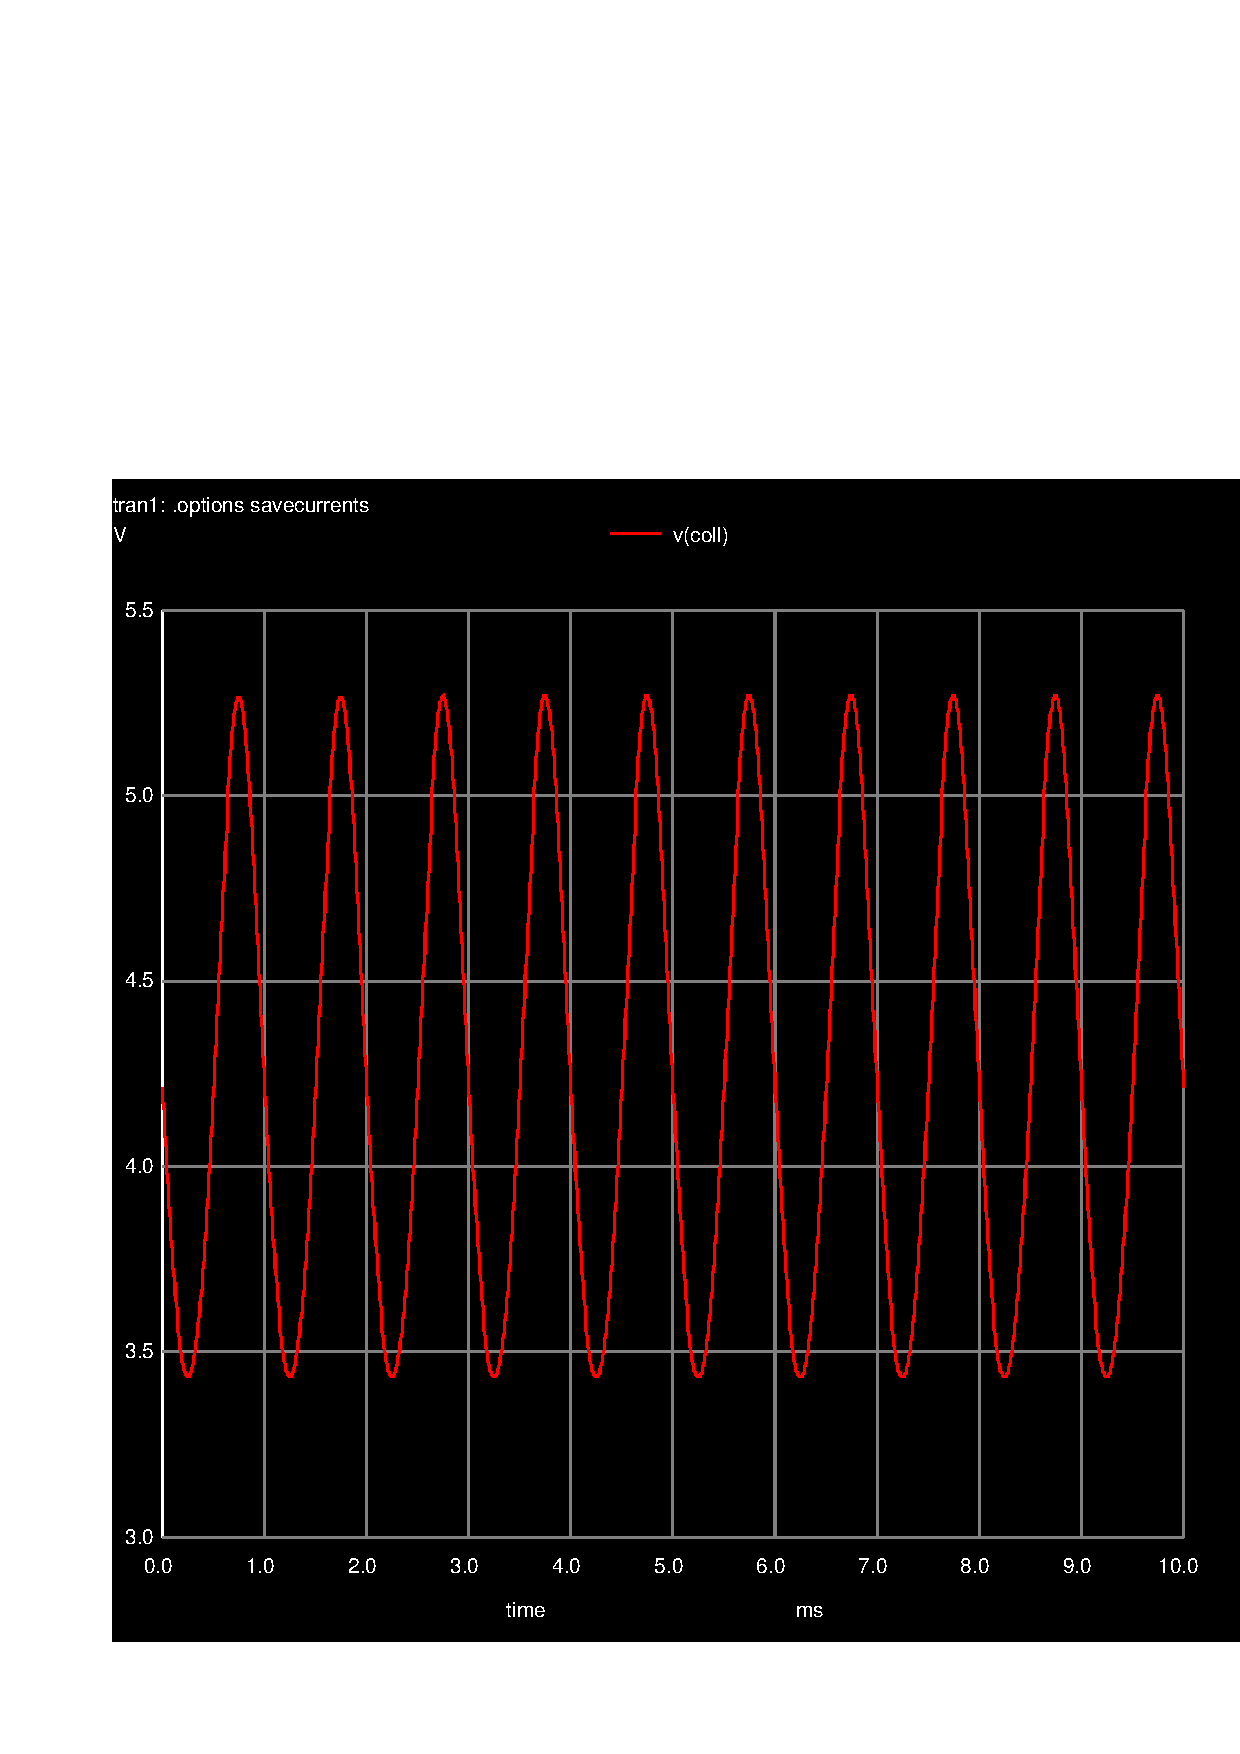
\includegraphics[width=0.45\linewidth]{vgs.pdf}
\caption{Gain Stage Output signal}
\label{fig:gain1}
\end{figure}

\vspace{-0.9in}
\begin{figure}[H] \centering
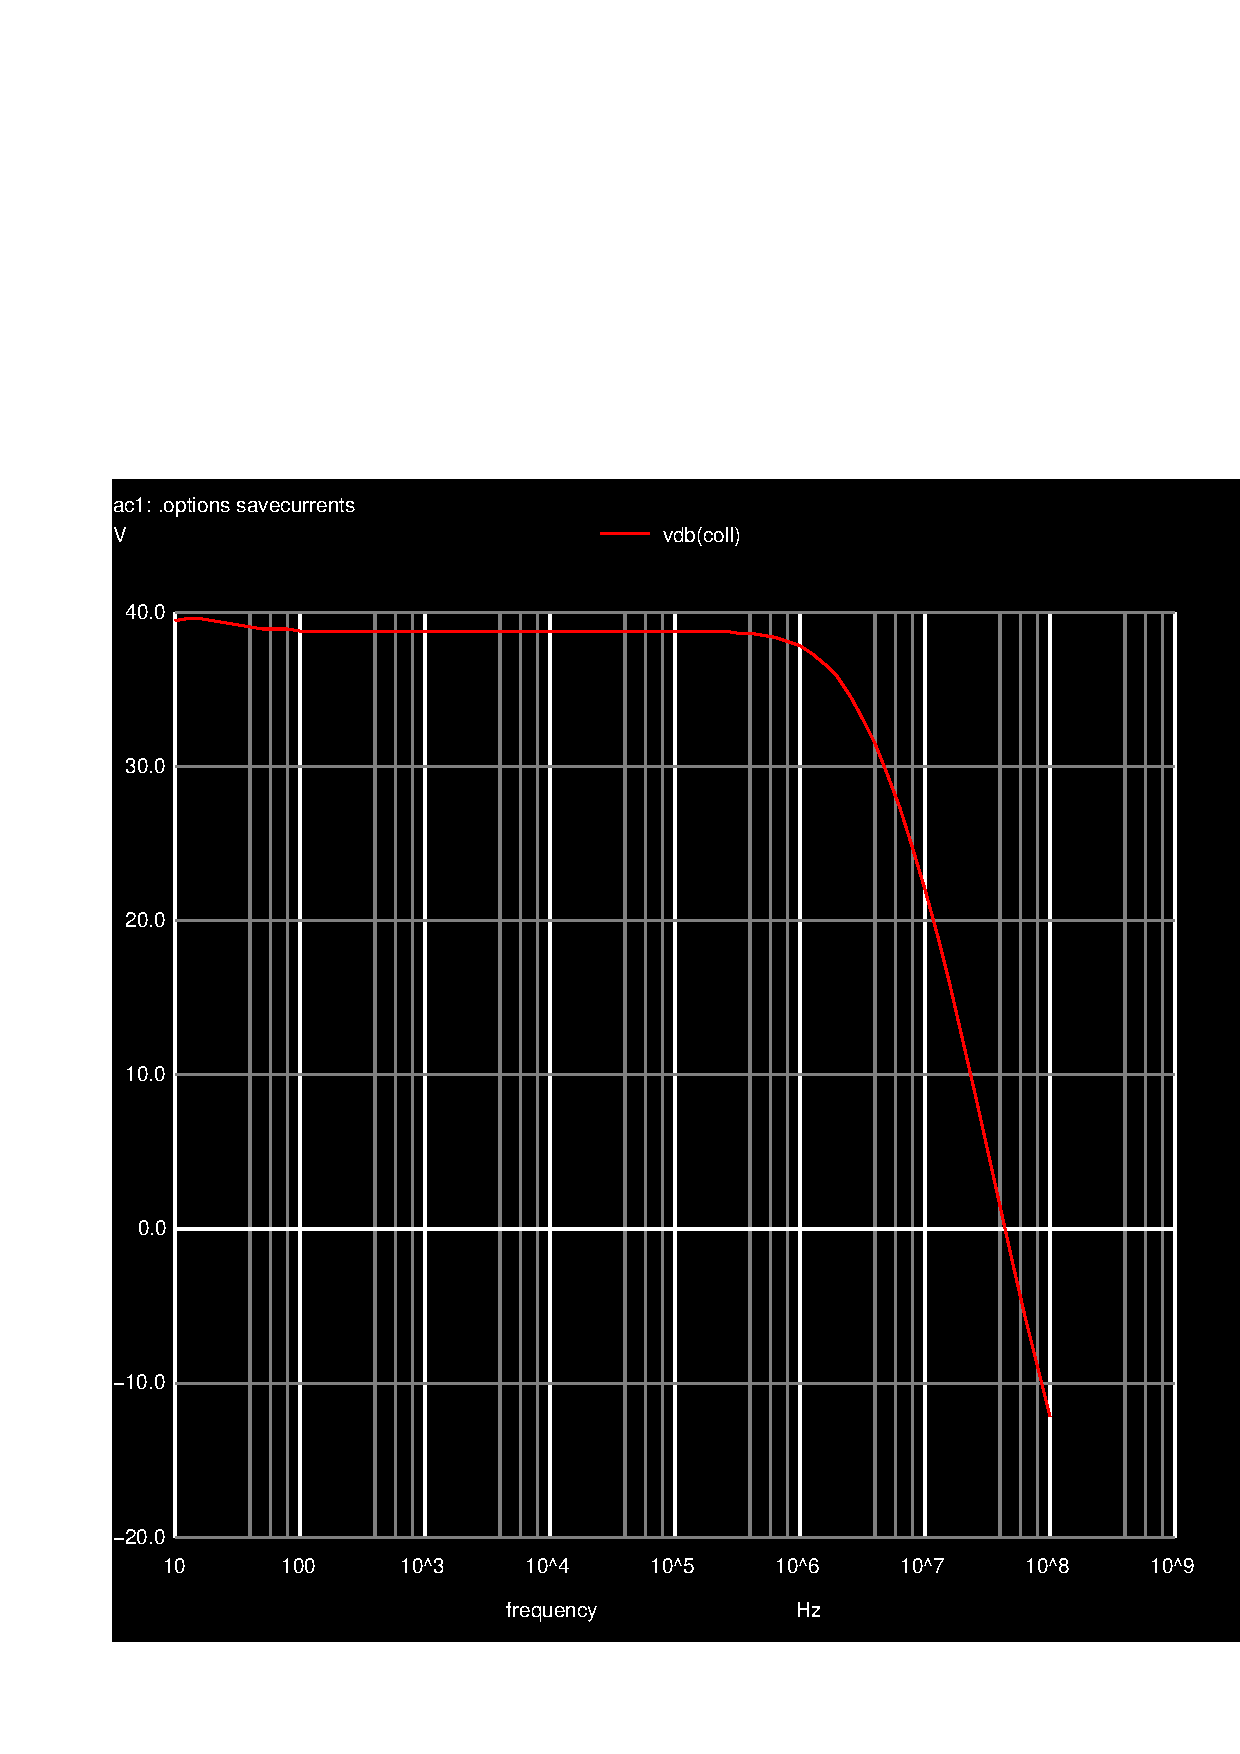
\includegraphics[width=0.45\linewidth]{vdbgs.pdf}
\caption{Gain Stage Output Gain}
\label{fig:gain2}
\end{figure}


\subsection{Output Stage}



The purpose of the Output Stage was to put an output impedance low enough so that the entire voltage gain would go to the audio speaker instead of getting lost in one of the resistors. In this way, it is intended that the gain stays approximately unchanged and that the output impedance has a value of at least one order of magnitude below the loudspeaker resistance. In the figure below we show the circuit configuration and its components. in the following table we present the values of each component.



\begin{figure}[H] \centering
\includegraphics[width=0.9\linewidth]{Output.pdf}
\caption{Output stage developed}
\label{fig:dev1}
\end{figure}


\begin{table}[ht]
  \centering
  \begin{tabular}{|l|r|}
    \hline    
    {\bf Name} & {\bf Value [V], [$\Omega$], [mF]} \\ \hline
    \input{oscircuitvalues_TAB}
  \end{tabular}
  \caption{Values of the components and  transistor parameters}
  \label{tab:r1}
\end{table}
\vspace{0.3in}

\subsubsection{Output Capacitor - $C_O$}

As it was expressed before, this Capacitor's purpose is to block the DC component and allow the passage of the AC component.


\subsubsection{Gain}

The second objective of this stage is to maintain the Gain value. That is, to make this stage have a gain very close to one. This objective was achieved, as can be seen in the side by side comparison, between the gain and output stage outputs. 


\subsection{Input and output impedance}

One of the fundamental points in our amplifier is that the input impedance must be much greater than the resistance of the signal source, so that, when the voltage division occurs, there are no significant losses. The other point is that the output impedance must be as low as possible compared to the resistance of our speaker, so that, once again, when the split of our output signal will occur, it goes almost entirely to the audio speaker.

In this way we were able to calculate these two circuit parameters.

\subsubsection{Input Impedance}

To compute the input impedance, we have calculated the resistance that is "seen" by the signal source. In this way, we divide the voltage at the output of the signal source resistance, for the current that passes in that branch: 



\begin{equation}
    Z_i = \frac{V(i_{n2})}{I(R_S)}
\end{equation}

We calculated this value for a frequency that is within the bandwidth interval. We also made the plot of the input impedance in relation to the frequency. We easily conclude that the impedance value in the bandwidth region is constant.


\vspace{0.1in}
\begin{table}[ht]
  \centering
  \begin{tabular}{|l|r|}
    \hline    
    {\bf Name} & {\bf Value [$k\Omega$]} \\ \hline
    \input{zingspice_tab}
  \end{tabular}
  \caption{Values of Input impedance}
  \label{tab:r2}
\end{table}
\vspace{0.3in}

\vspace{-0.9in}
\begin{figure}[H] \centering
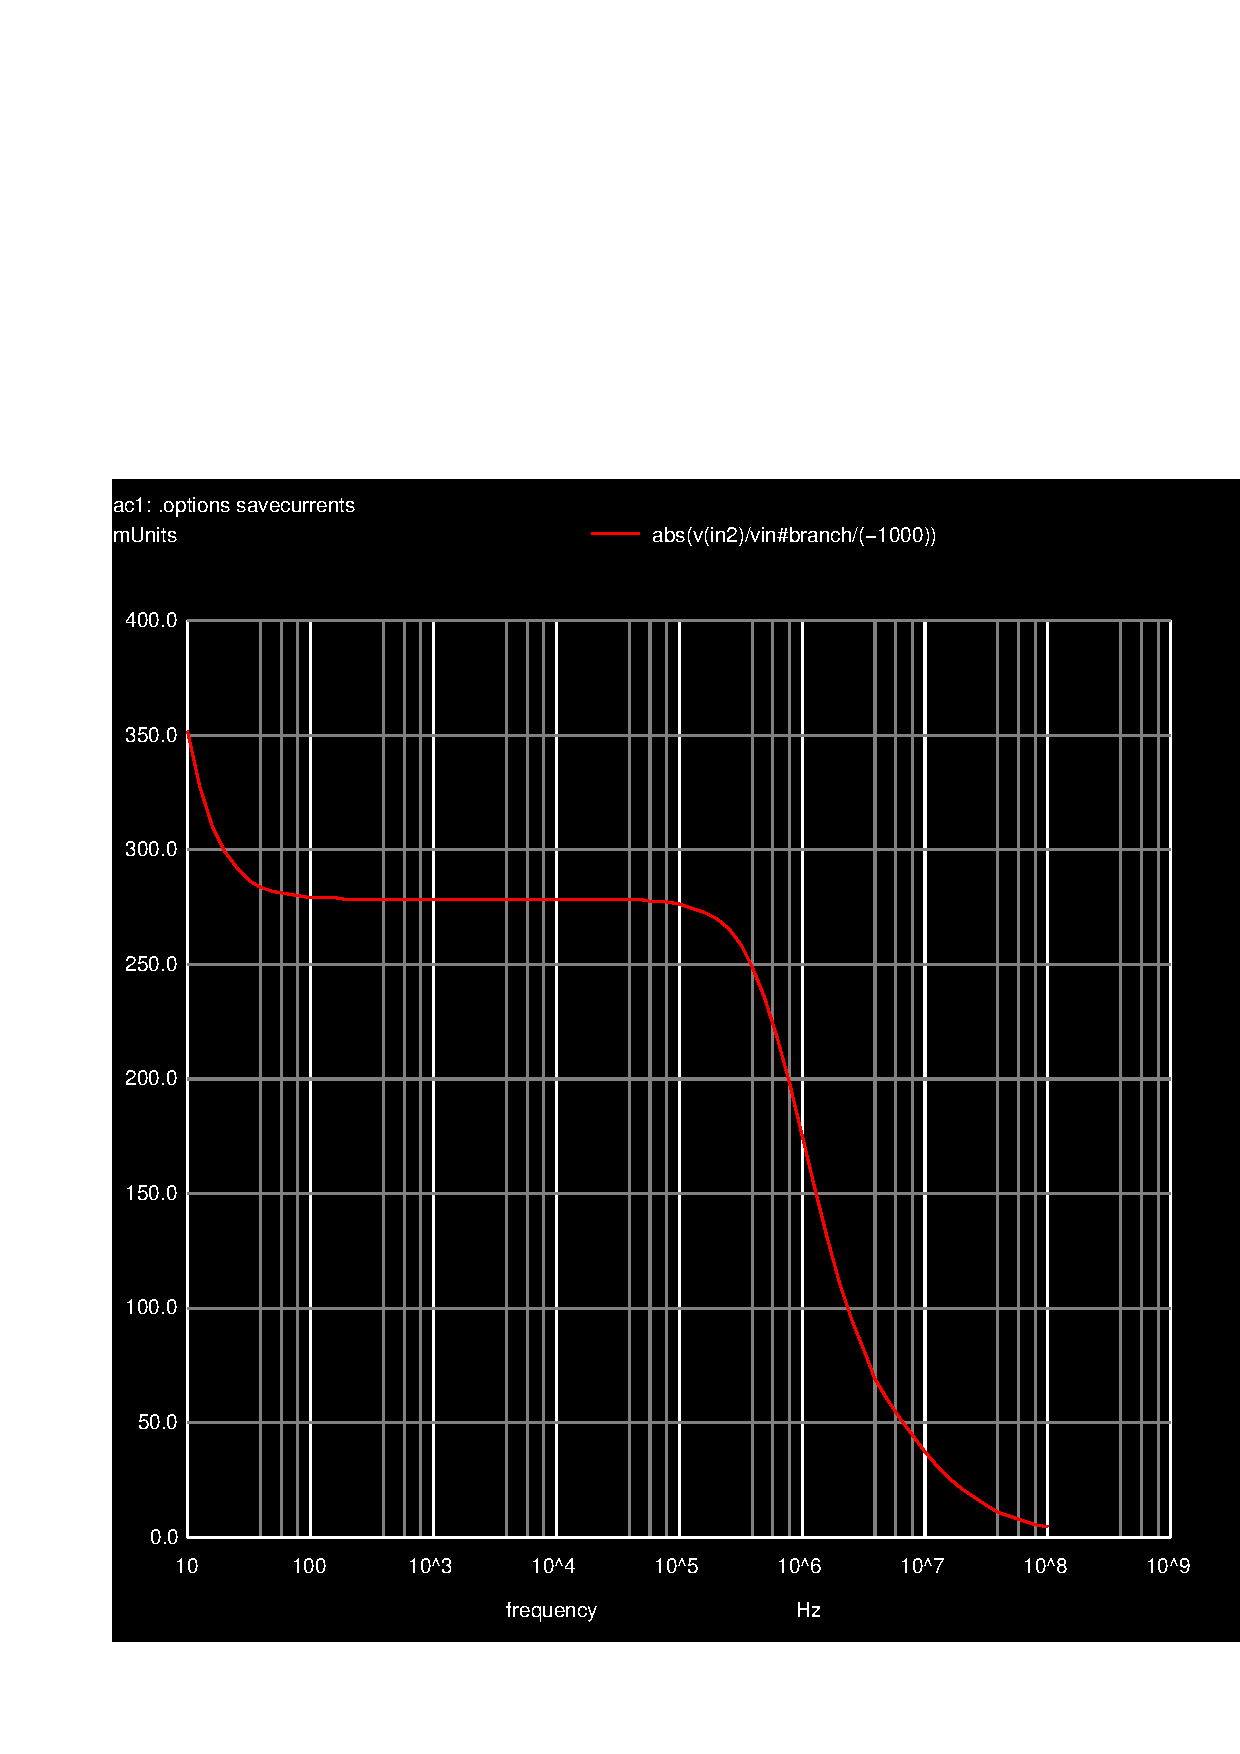
\includegraphics[width=0.45\linewidth]{zi.pdf}
\caption{Zi in function of frequency}
\label{fig:dev122}
\end{figure}

\subsubsection{Output Impedance}


To compute the output impedance, we only used the output stage. This can be done because there is no retroactivity, so the $Z_O$ of the output stage is almost equal to the $Z_O$ of the hole circuit. We proceeded in a similar way: first we turned off the signal source, then we put a voltage source in the place of the speaker resistance, and from the voltage and current in that branch, we determined the $Z_O$. Also, as in the input, we made the plot in function of the frequency. We quickly notice that $Z_O$ is minimal and constant in the bandwith. This is in accordance with the gain behavior, which increases when the $Z_O$ is smaller, that is, the voltage divider causes most of the signal to go to the load resistance.


\begin{equation}
    Z_O = \frac{V(out)}{I(out)}
\end{equation}


\vspace{0.1in}
\begin{table}[ht]
  \centering
  \begin{tabular}{|l|r|}
    \hline    
    {\bf Name} & {\bf Value [$k\Omega$]} \\ \hline
    \input{zongspice_tab}
  \end{tabular}
  \caption{Value of output impedance}
  \label{tab:r3}
\end{table}
\vspace{0.3in}

\vspace{-0.9in}
\begin{figure}[H] \centering
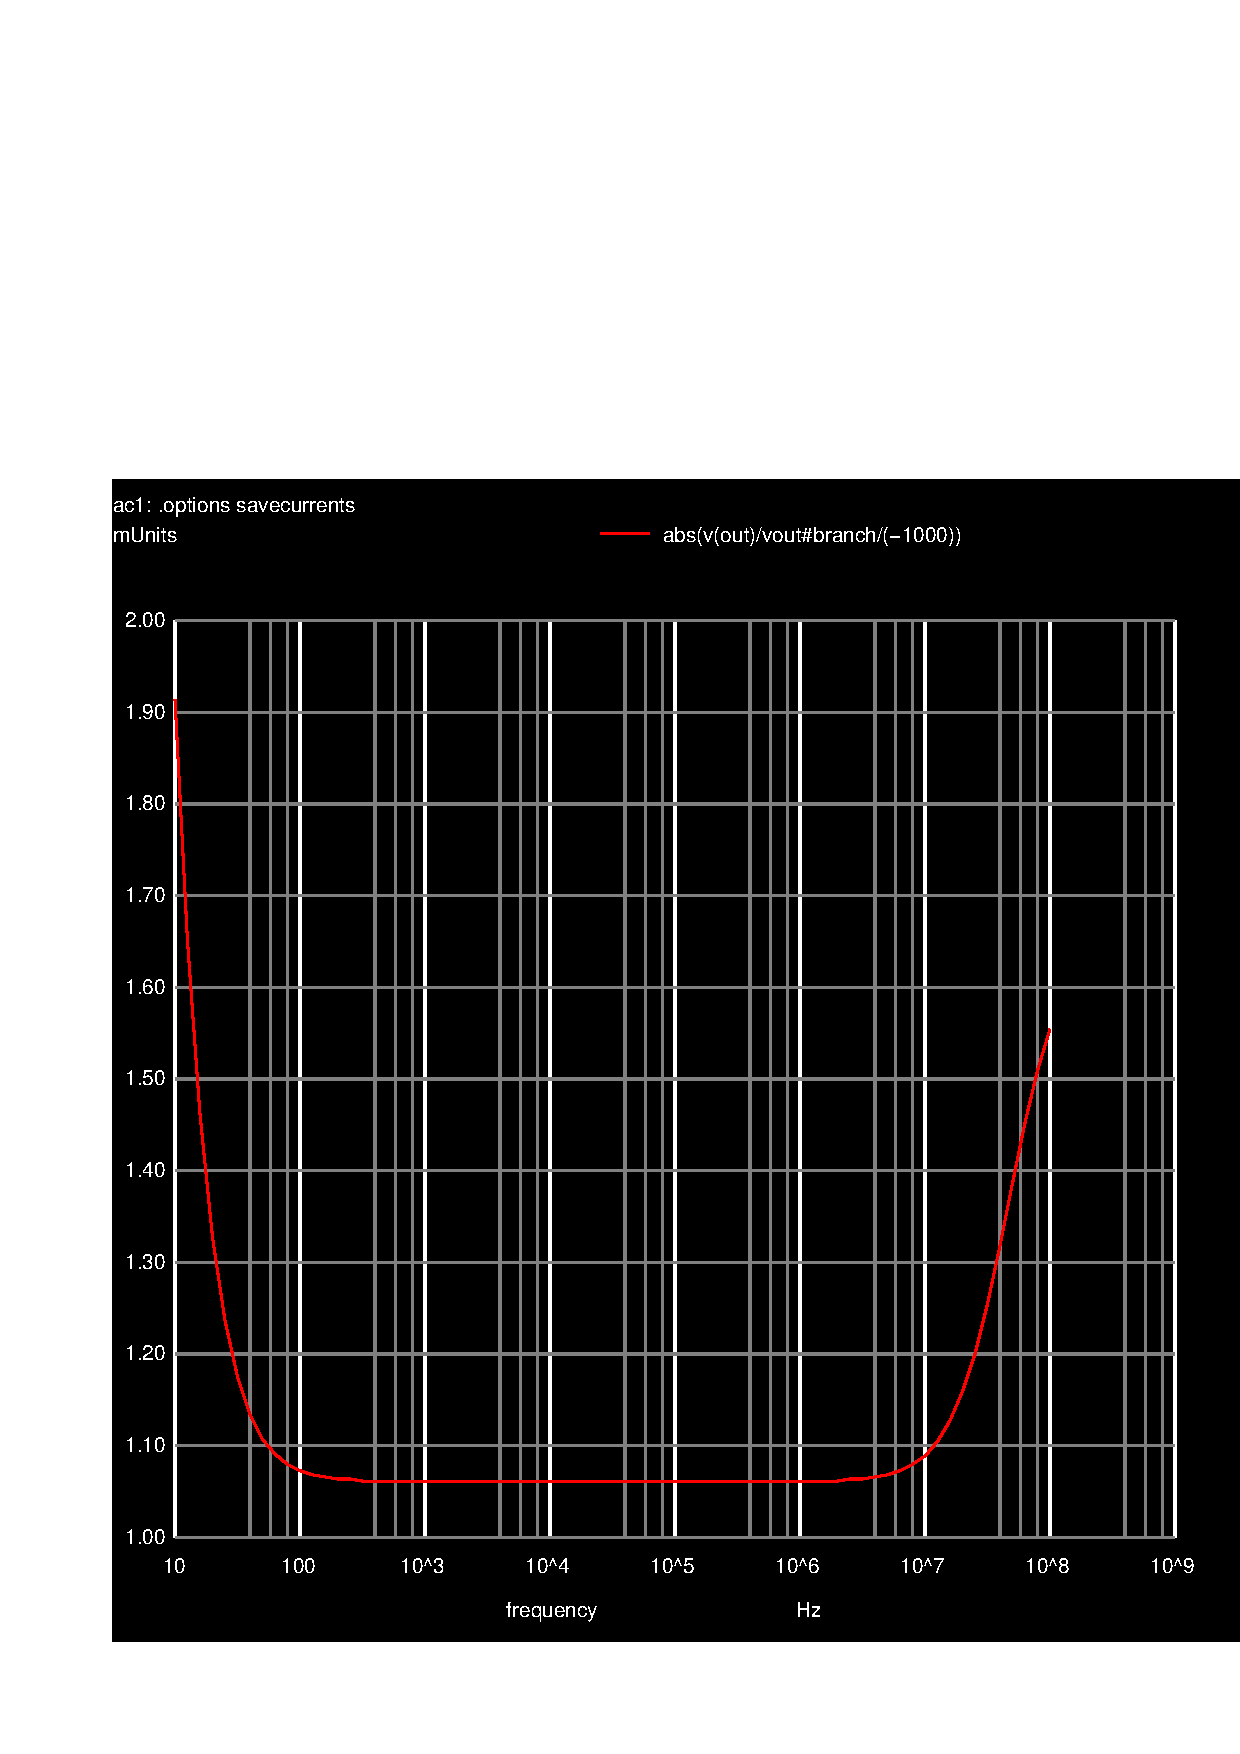
\includegraphics[width=0.45\linewidth]{zo.pdf}
\caption{Output impedance in function of frequency}
\label{fig:dev3}
\end{figure}

\newpage
\subsection{Final Result}

After the two stages were connected, the simulated behavior was the one expected, that is, the signal was amplified and was not distorted:



\begin{figure}[H] \centering
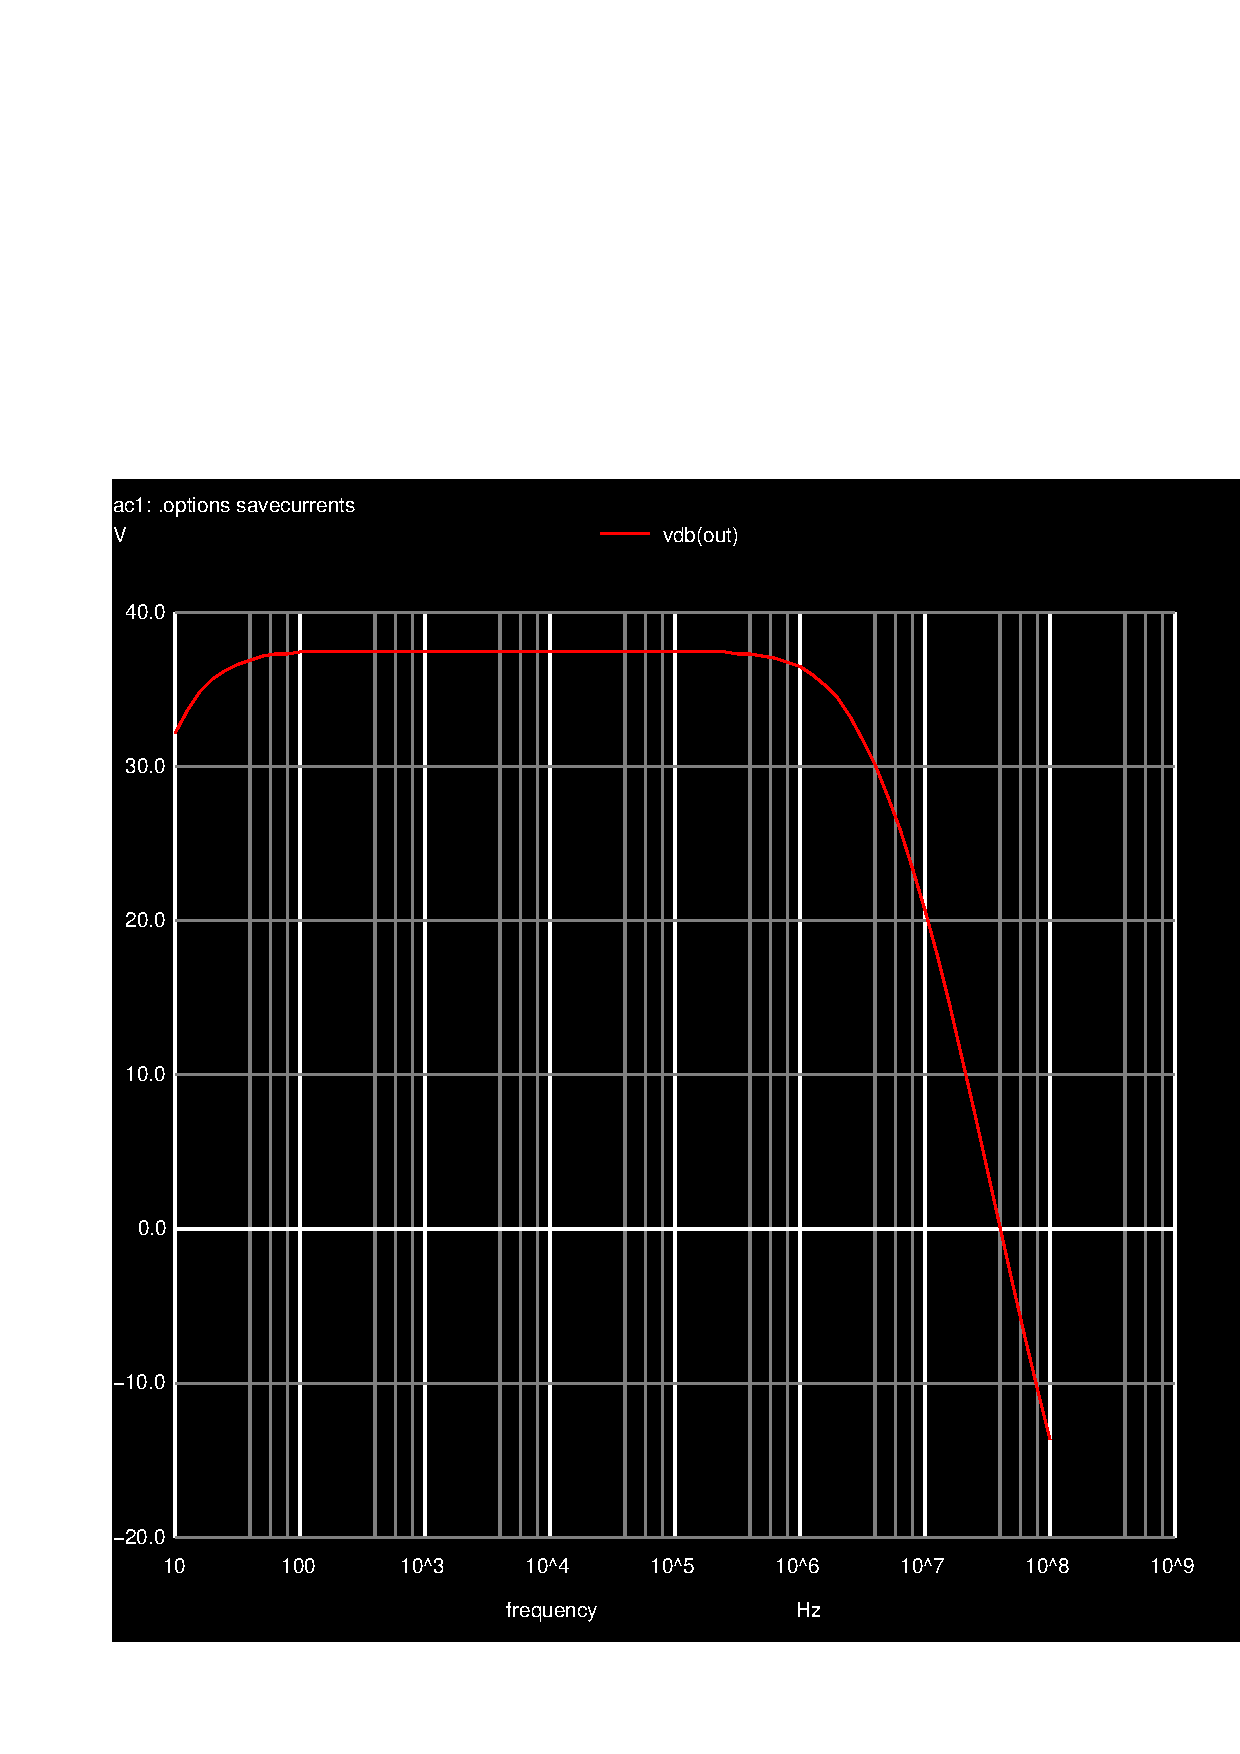
\includegraphics[width=0.45\linewidth]{vdbout.pdf}
\caption{Audio amplifier Gain}
\label{fig:dev4}
\end{figure}

With the important data for this lab to be the data shown below:


\vspace{0.1in}
\begin{table}[ht]
  \centering
  \begin{tabular}{|l|r|}
    \hline    
    {\bf Name} & {\bf Value [dB] [Hz]} \\ \hline
    vdboutmax & 3.744713e+01\\ \hline
freq_atl & 1.480389e+01\\ \hline
freq_atu & 1.981780e+06\\ \hline
freq_atu - freq_atl & 1.981765e+06\\ \hline
vdboutmax * ( freq_atu - freq_atl ) / freq_atl & 5.012967e+06\\ \hline

  \end{tabular}
  \caption{Values of interest}
  \label{tab:r4}
\end{table}
\vspace{0.3in}

The Gain was determined from the maximum value of the gain as a function of frequency plot. The lower and upper cutoff frequencies were determined from the find function, when the gain dropped by 3dB in relation to the maximum.

\newpage


